% LipScribe -- Progress Report 2 (Weeks 1 and 2)
% Compile: pdflatex progress_report_weeks1-2.tex   (or: tectonic progress_report_weeks1-2.tex)
% Figures are in figures/; lipscribe-report.sty is copied from 3_project_management/milestone_docs.
\documentclass[11pt,a4paper]{article}
\usepackage{lipscribe-report}
\usepackage{graphicx}
\usepackage{amsmath}
\usepackage{float}
\usetikzlibrary{arrows.meta}
\fancyhead[L]{\small\sffamily\color{lsgrey}LipScribe -- Progress Report 2 (Weeks 1--2)}

\newcommand{\notstarted}{\textcolor{lsplan}{\sffamily Not started}}
\newcommand{\blocked}{\textcolor{red!60!black}{\sffamily\bfseries Blocked}}
\newcommand{\code}[1]{\texttt{\small #1}}
% \tile{big number}{explanation}
\newcommand{\tile}[2]{\colorbox{lslight}{\parbox[t][1.45cm][t]{0.212\textwidth}{\sffamily\raggedright
  {\Large\bfseries\color{lsblue}#1}\par\vspace{3pt}{\scriptsize\linespread{1.0}\selectfont #2\par}}}}
% ragged-right fixed-width column (no hyphenated words in narrow cells)
\newcolumntype{L}[1]{>{\raggedright\arraybackslash}p{#1}}
\setlength{\textfloatsep}{10pt plus 2pt minus 2pt}
\setlength{\floatsep}{8pt plus 2pt minus 2pt}
\setlist{itemsep=1pt,topsep=2pt,parsep=0pt}

\begin{document}

\docheader{Progress Report 2}{Weeks 1 and 2: set-up, data verification and the preprocessing pipeline}{29 October 2026}

% =====================================================================
\section{Summary}
In the first two weeks (19--29 October) the team completed all of Week~1 and
most of Week~2. The GRID corpus is downloaded and verified on the team's GPU
workstation, split by speaker, and feeds a tested pipeline that turns each
utterance into mouth crops, 16\,kHz audio mixed with noise and a CTC target,
batched and ready for training. The first model component, the audio encoder,
is finished and tested, so every part of the audio-only baseline (B1) now
exists. Milestone M1 is closed; Milestone M2 (due Sunday 1~November) is open
because the full mouth-crop extraction (W2-02) still has to run over all 33
usable speakers and B1 has not yet started training. The figures in this report
come from the repository, its test suite and the integrity report produced on
the workstation, not from the Trello board alone.

\medskip
\noindent\tile{22 / 26}{task cards done (Week 1: 12 of 12, Week 2: 10 of 14)}\hfill%
\tile{96.7\,\%}{of 34,000 utterances pass every integrity check}\hfill%
\tile{160 / 163}{tests pass on \emph{main}; the rest need workstation clips}\hfill%
\tile{25 / 28}{merged pull requests have a recorded review}

\begin{figure}[H]
\centering
\begin{tikzpicture}[yscale=0.9,
  box/.style={draw, rounded corners=2pt, align=center, font=\sffamily\scriptsize,
              minimum height=0.95cm, inner sep=2pt, line width=0.6pt},
  done/.style={box, fill=lsdone!10, draw=lsdone, text width=2.35cm},
  prog/.style={box, fill=lsprog!14, draw=lsprog, text width=2.35cm},
  inp/.style={box, fill=lslight, draw=lsblue, text width=1.6cm},
  mdone/.style={done, minimum height=0.72cm},
  mtodo/.style={box, fill=white, draw=lsgrey, dashed, minimum height=0.72cm},
  arr/.style={-{Stealth[length=3.5pt]}, black!65, line width=0.6pt}]
  \def\st#1#2{\\[-1pt]{\tiny\color{#1}#2}}
  % data pipeline: three input rows (input -> first stage -> second stage)
  \foreach \yy/\xn/\xin/\xa/\xak/\xac/\xat/\xb/\xbk/\xbc/\xbt in {
      2.6/v/{GRID video\\(25 fps)}/{\textbf{Mouth crops}\\Face Mesh, 96$\times$96}/done/lsdone/done/{\textbf{Full-corpus run}\\(W2-02)}/prog/lsprog/in progress,
      1.3/a/{GRID audio\\(25 kHz)}/{\textbf{16 kHz mono}\\conversion}/done/lsdone/done/{\textbf{Noise mixing}\\+ $-$25 dBFS level}/done/lsdone/done,
      0/t/{Word\\alignments}/{\textbf{Transcript}\\\textbf{parser}}/done/lsdone/done/{\textbf{Tokeniser}\\28 symbols}/done/lsdone/done} {
    \node[inp] (i\xn) at (0.85,\yy) {\xin};
    \node[\xak] (a\xn) at (3.35,\yy) {\xa\st{\xac}{\xat}};
    \node[\xbk] (b\xn) at (6.25,\yy) {\xb\st{\xbc}{\xbt}};
    \draw[arr] (i\xn) -- (a\xn);
    \draw[arr] (a\xn) -- (b\xn);
  }
  \node[done, text width=1.45cm, minimum height=3.4cm] (m) at (9.0,1.3)
       {\textbf{Manifest}\\\textbf{split}\\\textbf{dataset}\\\textbf{collate}\st{lsdone}{done}};
  \foreach \xn in {v,a,t} \draw[arr] (b\xn.east) -- (b\xn.east -| m.west);
  % model and training column: visual encoder left, audio branch right
  \node[mdone, text width=1.95cm] (f) at (15.25,3.25) {\textbf{Audio features}\st{lsdone}{done (W2-07)}};
  \node[mtodo, text width=1.95cm] (ve) at (13.05,2.1) {\textbf{Visual encoder}\st{lsgrey}{Week 3 (W3-03)}};
  \node[mdone, text width=1.95cm] (ae) at (15.25,2.1) {\textbf{Audio encoder}\st{lsdone}{done (W2-11)}};
  \node[mtodo, text width=4.15cm] (fu) at (14.15,0.95) {\textbf{Attention fusion} (model P)\st{lsgrey}{planned: Week 4}};
  \node[mdone, text width=4.15cm] (c) at (14.15,-0.2) {\textbf{CTC head + greedy decoder}\st{lsdone}{done (W2-12)}};
  \node[mdone, text width=4.15cm] (tr) at (14.15,-1.35) {\textbf{train.py + WER / CER}\st{lsdone}{done (W2-13)}};
  \draw[arr] (m.east |- f) -- (f.west);
  \draw[arr] (m.east |- ve) -- (ve.west);
  \draw[arr] (f) -- (ae);
  \draw[arr] (ae) -- (ae |- fu.north);
  \draw[arr] (ve) -- (ve |- fu.north);
  \draw[arr] (fu) -- (c);
  \draw[arr] (c) -- (tr);
  \node[font=\sffamily\scriptsize\bfseries, text=lsblue, anchor=west] at (0.1,4.05) {Data pipeline};
  \node[font=\sffamily\scriptsize\bfseries, text=lsblue, anchor=west] at (11.9,4.05) {Model and training};
\end{tikzpicture}
\caption{The LipScribe pipeline and the status of each stage on 29 October. All
data stages are built and tested except the full-corpus crop run; every part of
B1 (audio encoder $\to$ CTC head) exists, and the visual encoder and fusion
follow in Weeks 3--4.}
\label{fig:pipeline}
\end{figure}

% =====================================================================
\section{Progress against the plan}

{\small
\rowcolors{2}{lsrow}{white}
\begin{tabularx}{\textwidth}{@{}XL{1.9cm}L{5.6cm}@{}}
\toprule
\rowcolor{white}\sffamily\bfseries Milestone & \sffamily\bfseries Due & \sffamily\bfseries Status \\
\midrule
M1 Environment and dataset verified & Sun 25 Oct & \done{} -- closed 29 Oct, 4 days late \\
M2 Preprocessing and alignment & Sun 1 Nov & \inprog{} -- 3 of 6 criteria met \\
M3 \& M4 Baselines B1, B2, B3 & Sun 8 Nov & \planned \\
M5 Multimodal fusion (model P) & Sun 15 Nov & \planned \\
M6 \& M7 Tuning and evaluation (core freeze) & Sun 22 Nov & \planned \\
M8 \& M9 Application, testing, demo & Sun 29 Nov & \planned \\
\bottomrule
\end{tabularx}
}

\medskip
M2 criteria met: crop contact sheets reviewed, noise-mixing tests pass, and one
batch loads with consistent lengths. Still to do: the train/inference parity
test, a running B1 job and the Week~3 re-plan. Most Trello cards were moved to
\emph{Done} in one update on 29 October, so the pull-request history
(Section~5) is the more reliable record of when work finished.

% =====================================================================
\section{Week 1: set-up and data (Milestone M1)}

{\small
\rowcolors{2}{lsrow}{white}
\begin{tabularx}{\textwidth}{@{}L{1.05cm}L{3.75cm}L{1.35cm}X@{}}
\toprule
\rowcolor{white}\sffamily\bfseries Card & \sffamily\bfseries Task & \sffamily\bfseries Owner & \sffamily\bfseries Output and evidence \\
\midrule
W1-01 & Kick-off, roles, Trello & Charis & Board: every card has an owner, reviewer, due date, checklist \\
W1-02 & Repository skeleton & Nehum & Package \code{lipscribe/}, one sub-package per stage (PR \#2) \\
W1-03 & Pinned environment & Nehum & \code{requirements.txt}, \code{environment.yml}, \code{check\_env.py} \\
W1-04 & GPU and storage & Charis & Linux GPU workstation (``Alienware'') runs all full-corpus jobs \\
W1-05 & Download GRID & Faith & 34 speakers $\times$ 1,000 utterances: video, audio, alignments \\
W1-06 & MUSAN noise pools & Lisa & Split \emph{by file} 70/15/15: test noise never heard in training \\
W1-07 & Integrity checker & Faith & \code{verify\_dataset.py}: 7 checks per utterance (Table~\ref{tab:integrity}) \\
W1-08 & Speaker split & Faith & \code{make\_splits.py}: fixed seed, refuses to overwrite \\
W1-09 & Tokeniser & Lisa & 28 symbols; verified on all 33,000 alignment files \\
W1-10 & Mouth-crop prototype & Cole & Face Mesh lip crops, 96$\times$96 grey; tested on five clips \\
W1-11 & Interface specification & Isabelle & \code{INTERFACES.md}: every function, key and shape (PR \#4) \\
W1-12 & Tests and CI & Nehum & pytest suite and a GitHub Actions file (PR \#6) \\
\bottomrule
\end{tabularx}
}

\smallskip
\code{docs/INTERFACES.md} fixed every module's inputs, outputs and tensor shapes
before the modules were written, so the data, model and application pairs could
build in parallel; the Week~2 integration relied on it directly.

\subsection{Dataset integrity}
\code{verify\_dataset.py} ran over all 34,000 utterances on the workstation.
Table~\ref{tab:integrity} gives the pass count for each check. Almost every
failure comes from two speakers: s21 is distributed with audio only (no video
or alignments), and 108 of s8's videos do not decode. Beyond these, one s4
video does not decode and one s28 clip fails the audio-level check. The Face
Mesh check (at least 90\,\% of frames detected) is built in and is fed by the
crop extraction of W2-02.

\begin{table}[htbp]
\centering\small
\caption{Integrity check results (\code{reports/integrity\_report.csv}, 34,000 utterances).}
\label{tab:integrity}
\rowcolors{2}{lsrow}{white}
\begin{tabularx}{\textwidth}{@{}XrrL{6.4cm}@{}}
\toprule
\rowcolor{white}\sffamily\bfseries Check (per utterance) & \sffamily\bfseries Pass & \sffamily\bfseries Rate & \sffamily\bfseries Notes \\
\midrule
Video, audio and alignment files present & 33,000 & 97.1\,\% & s21: no video or alignment \\
Video decodes & 32,891 & 96.7\,\% & s8: 108 $\cdot$ s4: 1 \\
Frame count $75 \pm 2$ & 32,891 & 96.7\,\% & 32,816 at 75 frames, 74 at 74 \\
Audio--video sync ($\le 40$\,ms) & 32,891 & 96.7\,\% & 20\,ms offset on every clip \\
Transcript is six valid GRID words & 33,000 & 97.1\,\% & 51 words; 20--31 characters \\
Audio not silent or clipped & 33,999 & 100.0\,\% & s28: 1 clip \\
\textbf{All checks} & \textbf{32,890} & \textbf{96.7\,\%} & 33 of 34 speakers usable \\
\bottomrule
\end{tabularx}
\end{table}

The report also revealed a property of this copy of GRID that the pipeline
must handle: the audio is \emph{end-pointed}. Each file holds only the spoken
part, 1.10--2.94\,s long (mean 1.83\,s), while every video lasts 3.0\,s, and
speech starts on average 0.47\,s (at most 1.51\,s) into the video. All files are
pre-levelled to $-26$\,dBFS. Without correction the audio would run ahead of the
lips; Section~4.7 describes the fix.

\subsection{Speaker-independent split}
Speakers, not utterances, are split, so no test speaker is ever heard or seen
in training (Figure~\ref{fig:split}). The test set has two female and two male
speakers and the validation set three speakers of both sexes; every other usable
speaker trains. The split was generated once with a fixed seed (2026) and is
committed; \code{make\_splits.py} refuses to overwrite it, and a test asserts
that the three speaker sets are pairwise disjoint.

\begin{figure}[htbp]
\centering
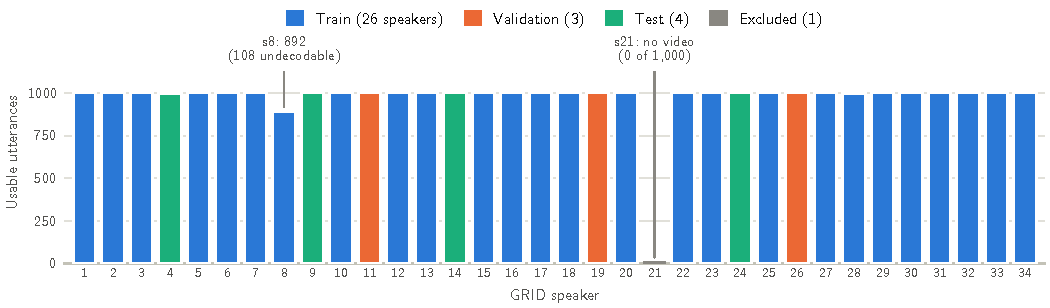
\includegraphics[width=\textwidth]{figures/speakers.pdf}
\caption{Usable utterances per GRID speaker after the integrity checks, coloured
by partition. Train: 26 speakers (14 male, 12 female), 25,891 utterances.
Validation: s11, s19, s26 (2 male, 1 female), 3,000. Test: s4, s9, s14, s24
(2 female, 2 male), 3,999. Excluded: s21.}
\label{fig:split}
\end{figure}

\subsection{Transcripts and tokeniser}
Transcripts come from the \code{.align} files with silence (\code{sil}) and
short pauses (\code{sp}) removed. The tokeniser maps them to 28 symbols:
blank~(0), space~(1) and the letters a--z (2--27). Lisa's
\code{verify\_tokenizer.py} checked it on all 33,000 real alignment files:
$\mathit{decode}(\mathit{encode}(s)) = s$ for every transcript, the blank is
never emitted, and the vocabulary holds the 51 GRID words. The longest
transcript is 31 characters (``place green with e eight please'') and the most
repeated adjacent letters in one transcript is 3. CTC therefore needs at most
$31 + 3 = 34$ output frames against 75 available per clip, so the CTC length
condition can never fail on GRID.

% =====================================================================
\section{Week 2: preprocessing and training pipeline (Milestone M2)}
Ten of the fourteen Week~2 cards are done (Table~\ref{tab:week2}); the four
open ones all wait on the full crop extraction or on B1 training.

\begin{table}[tbp]
\centering\small
\caption{Week 2 cards and their status on 29 October.}
\label{tab:week2}
\rowcolors{2}{lsrow}{white}
\begin{tabularx}{\textwidth}{@{}L{1.05cm}L{4.0cm}L{1.35cm}L{1.75cm}X@{}}
\toprule
\rowcolor{white}\sffamily\bfseries Card & \sffamily\bfseries Task & \sffamily\bfseries Owner & \sffamily\bfseries Status & \sffamily\bfseries Output and evidence \\
\midrule
W2-01 & Crop failure handling & Cole & \done & Failed frames interpolated, never dropped \\
W2-02 & Full mouth extraction & Faith & \inprog & Script merged; s1 pilot run done \\
W2-03 & Crop contact sheets & Isabelle & \done & Six speakers reviewed (Figure~\ref{fig:crops}a) \\
W2-04 & Audio to 16\,kHz & Lisa & \done & 34,000 of 34,000 files, 0 failures \\
W2-05 & Noise mixer & Lisa & \done & SNR within 0.01\,dB of target (PR \#22) \\
W2-06 & Fixed noisy val/test sets & Lisa & \done & \code{make\_noisy\_test.py} (PR \#22) \\
W2-07 & Feature extraction & Charis & \done & Matches librosa to $4.9\times10^{-5}$ \\
W2-08 & Normalisation statistics & Faith & \notstarted & Needs the crops from W2-02 \\
W2-09 & Manifest, dataset, collate & Charis & \done & Batch of 16 loads (PR \#18, \#21) \\
W2-10 & Parity test & Nehum & \inprog & Needs the crops from W2-02 \\
W2-11 & Audio encoder & Cole & \done & 5 of 5 tests pass (PR \#27) \\
W2-12 & CTC head, decoder, metrics & Isabelle & \done & Corpus-level WER/CER (PR \#13) \\
W2-13 & Training script & Charis & \done & Trains, saves, resumes and logs \\
W2-14 & GPU memory, B1 overfit & Charis & \planned & Unblocked by W2-11 \\
\bottomrule
\end{tabularx}
\end{table}

\subsection{Mouth crops}
MediaPipe Face Mesh finds the lip landmarks in every frame. A square box around
them, enlarged by 25\,\%, is smoothed with a centred five-frame moving average
and resized to 96$\times$96 grey pixels. When detection fails, the box is
interpolated from the nearest good frames and the frame is marked invalid in a
per-frame mask; frames are never dropped, so the video stays aligned with the
audio. A clip with more than 10\,\% invalid frames is excluded
(Figure~\ref{fig:crops}b). On the speaker-1 pilot run (1,000 clips) every clip
was cropped without error and 984 had all 75 frames detected; the average
failure rate was 0.19\,\% of frames, and 11 clips (1.1\,\%) exceeded the 10\,\%
limit. The crop review (W2-03) produced contact sheets for six speakers (s1, s2,
s10, s20, s30, s34; 140 sampled frames, all detected) and kept the 25\,\% margin
and five-frame smoothing unchanged. \code{extract\_mouths.py} runs the same
code over the whole corpus in one command, in parallel across all CPU cores,
and can be stopped and restarted without losing work; it writes the Face Mesh
report that \code{verify\_dataset.py} reads.

\begin{figure}[htbp]
\centering
\begin{minipage}[t]{0.33\textwidth}\vspace{0pt}
  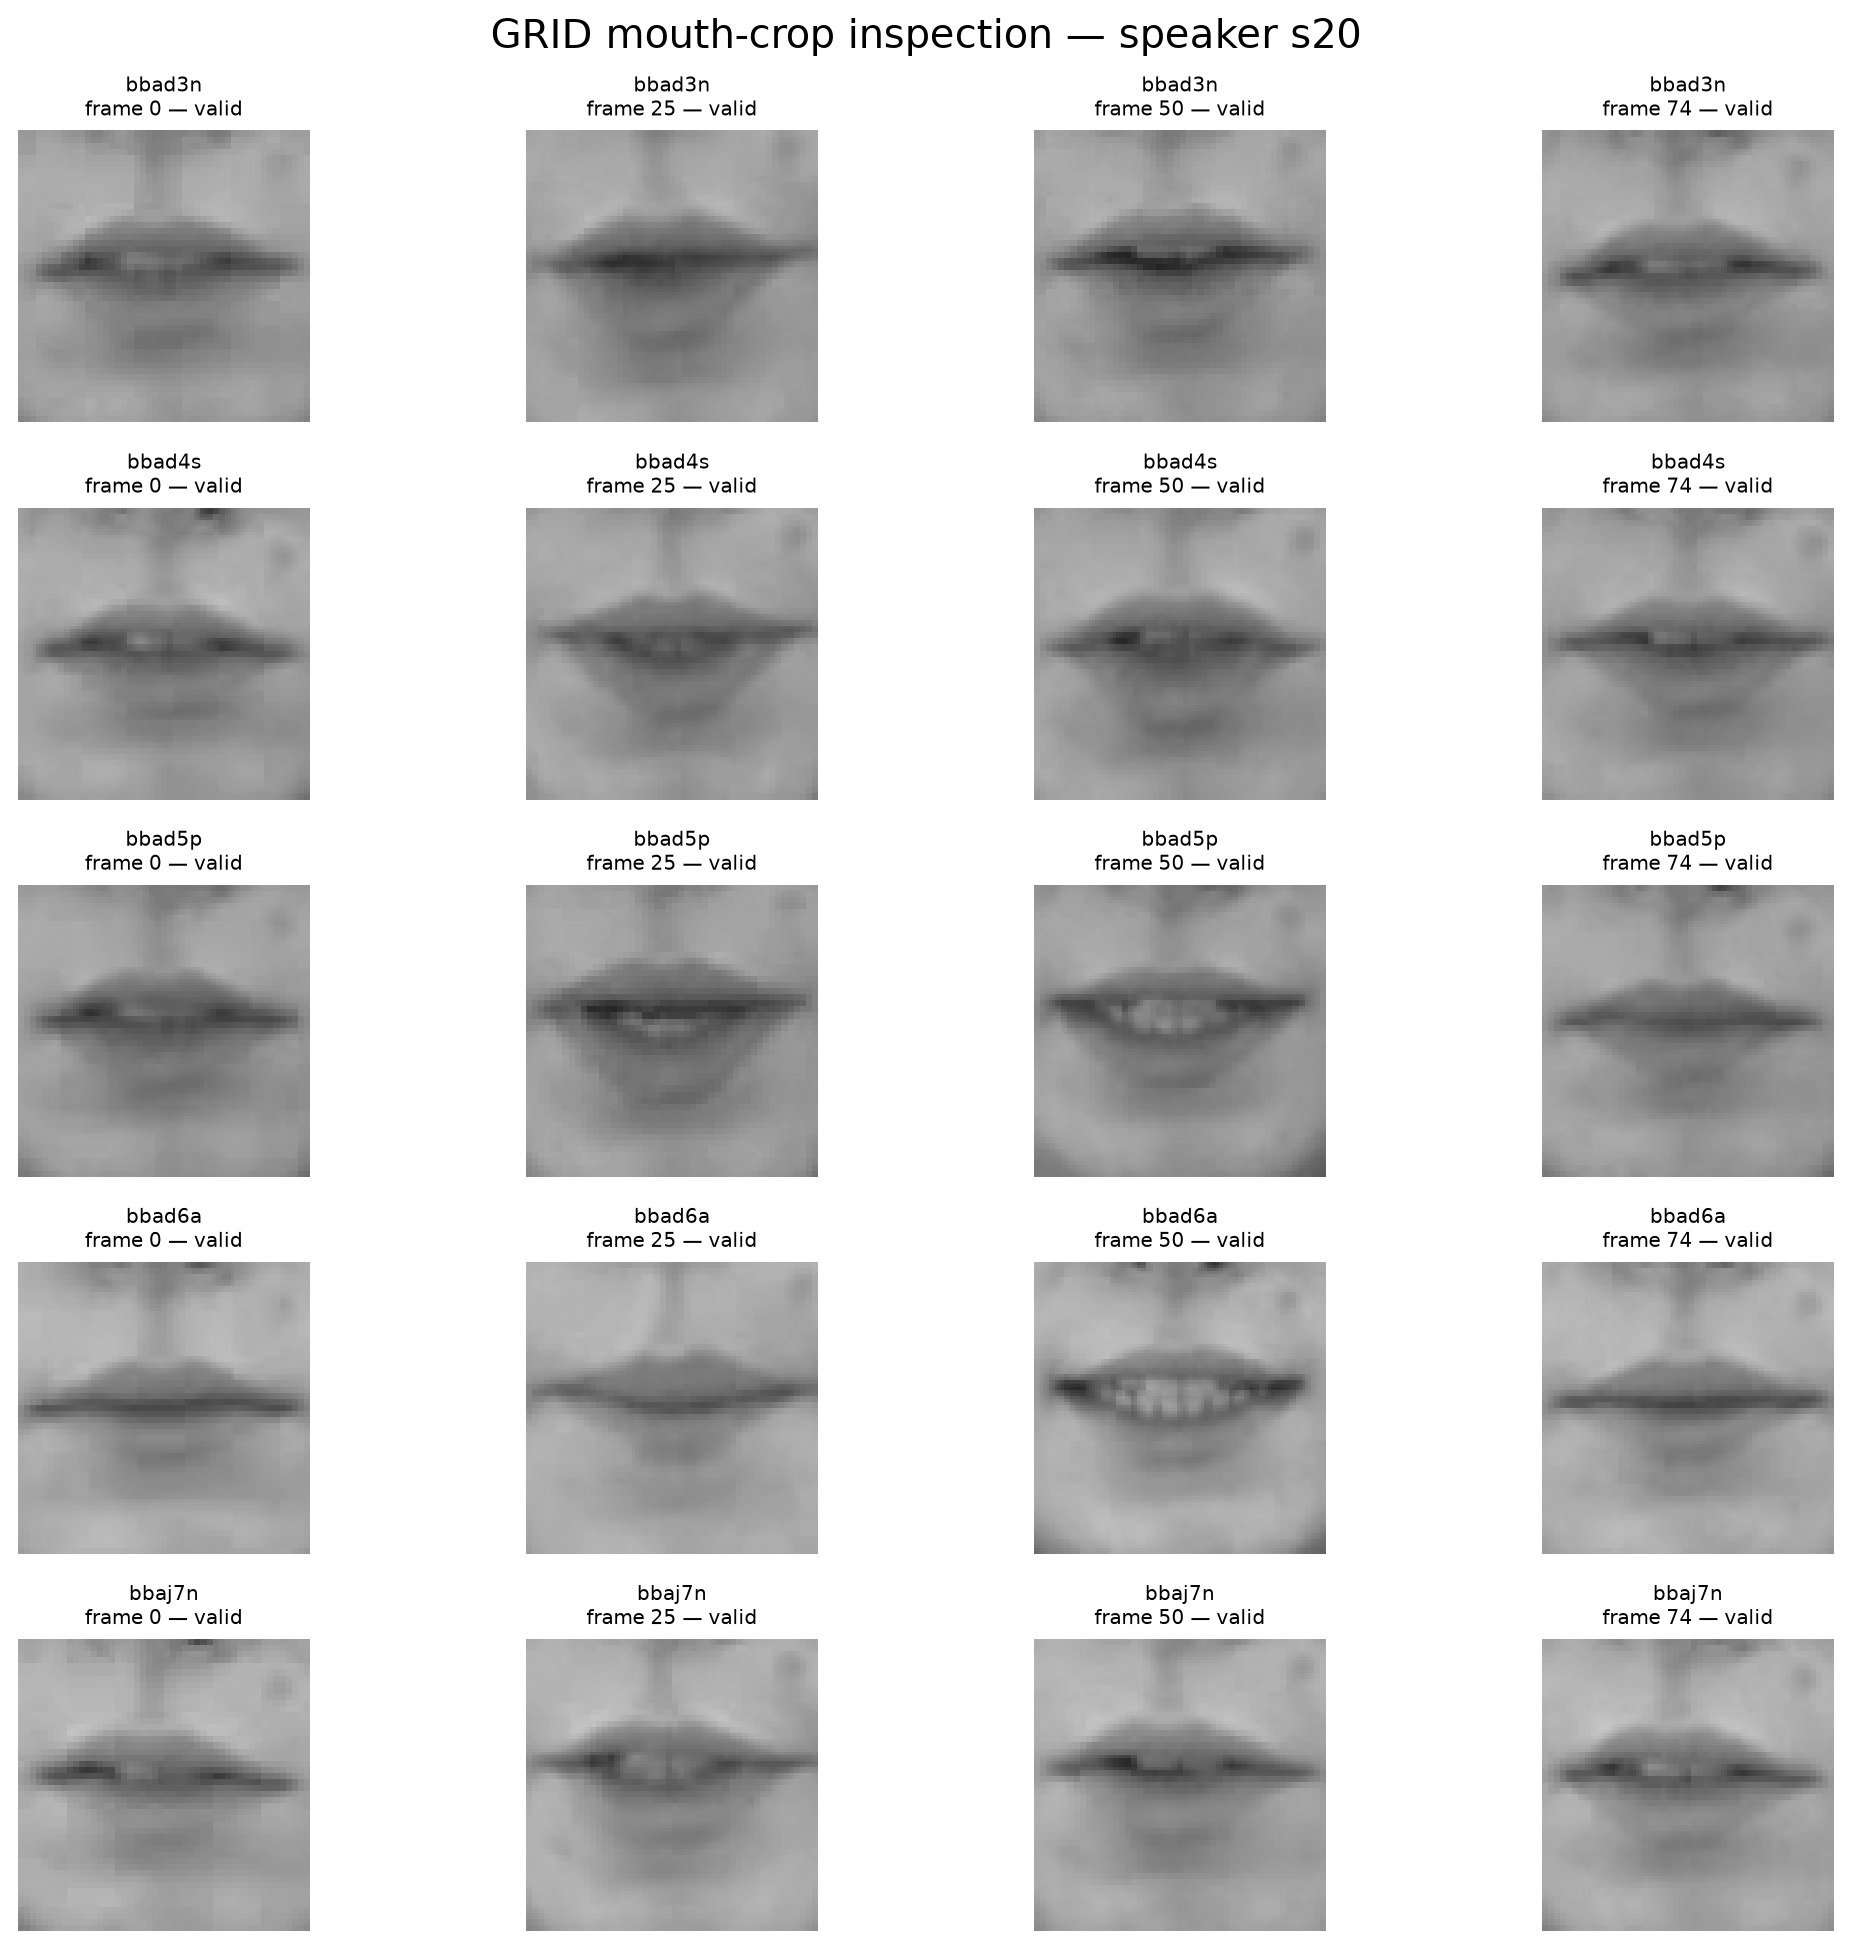
\includegraphics[width=\linewidth]{figures/s20_contact_sheet.png}
\end{minipage}\hfill
\begin{minipage}[t]{0.64\textwidth}\vspace{0pt}
  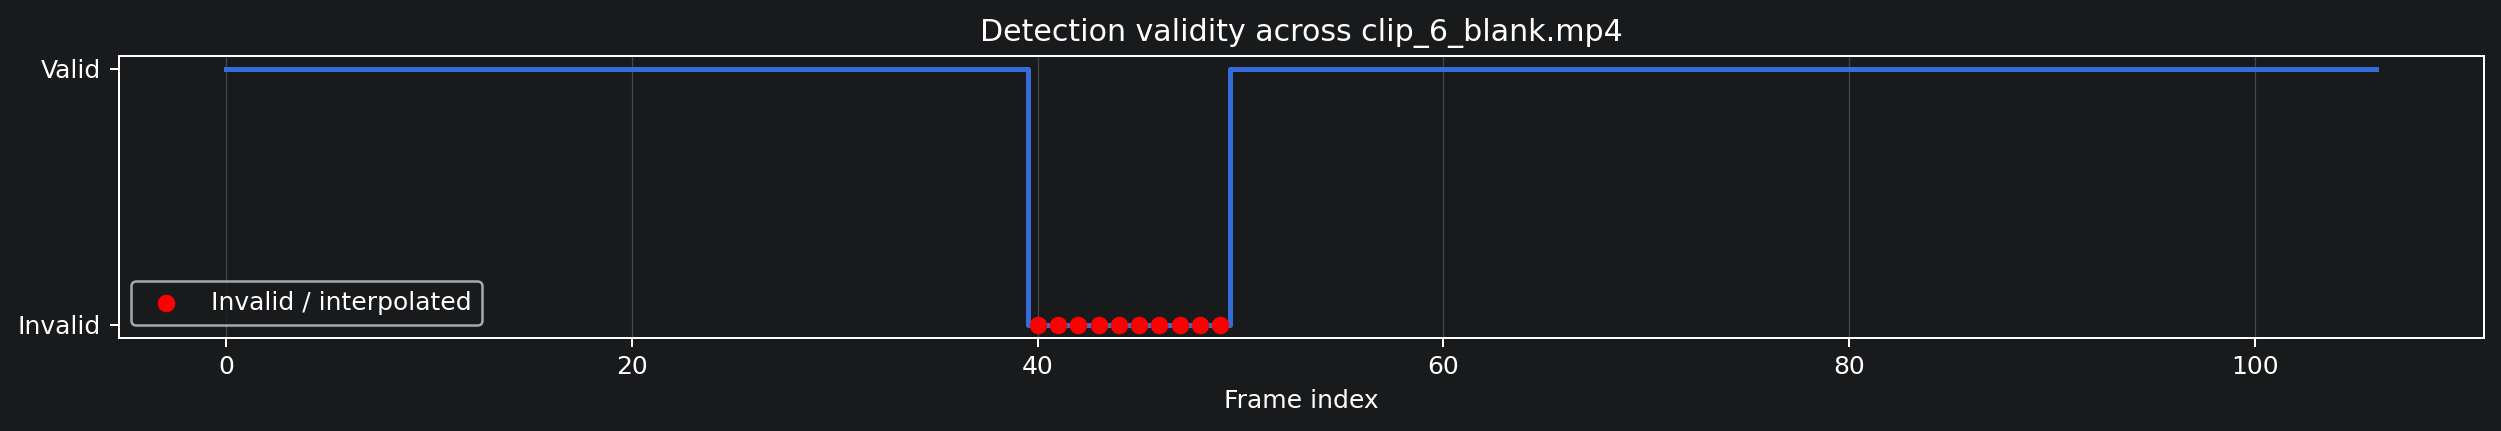
\includegraphics[width=\linewidth]{figures/clip6_validity.png}
  \captionof{figure}{(a, left) Contact sheet for speaker s20: frames 0, 25, 50
  and 74 of five utterances, all detected and centred on the mouth. (b, above)
  Failure handling on a test clip with frames 40--49 blanked out: those frames
  are marked invalid and their crop box is interpolated from the neighbouring
  frames, while the clip keeps every frame.}
  \label{fig:crops}
\end{minipage}
\end{figure}

\subsection{Audio and noise}
All GRID audio is converted to 16\,kHz mono, 16-bit WAV (34,000 files, no
failures). Noise from the MUSAN pools is added at a chosen signal-to-noise
ratio by scaling it by
$\alpha = \sqrt{P_s / (P_w \cdot 10^{\mathrm{SNR}/10})}$, where $P_s$ and $P_w$
are the speech and noise powers over the whole clip; the measured SNR is
checked to within 0.01\,dB, short noise is looped, and a mixture that would clip
is scaled down as a whole, which preserves the SNR. Training draws an SNR
uniformly from \{clean, 10, 5, 0, $-5$\}\,dB for every utterance; validation
and test use fixed pre-mixed files so every model hears identical audio. After
mixing each clip is levelled to $-25$\,dBFS, with the gain capped at $+20$\,dB.

\subsection{Audio features}
One shared module computes the features for both training (on the GPU, in
batches) and the demo app (one clip at a time). The configuration switch
\code{audio\_features} selects one of three feature sets
(Table~\ref{tab:features}). All use a 25\,ms Hann window, 10\,ms hop, 512-point
FFT and 80 Mel bands between 20\,Hz and 8\,kHz, with $\log(x + 10^{-6})$, and
give exactly four feature frames per video frame (300 for a 3\,s clip). The
log-Mel output matches \code{librosa} to $4.9 \times 10^{-5}$.

\begin{table}[htbp]
\centering\small
\caption{Audio feature configurations.}
\label{tab:features}
\rowcolors{2}{lsrow}{white}
\begin{tabularx}{\textwidth}{@{}L{1.2cm}L{2.6cm}XL{2.4cm}@{}}
\toprule
\rowcolor{white}\sffamily\bfseries ID & \sffamily\bfseries Config value & \sffamily\bfseries Features & \sffamily\bfseries Shape (3\,s) \\
\midrule
A1 & \code{logmel80} & 80 log-Mel bands (default; used by B1, B3, P) & [300, 80] \\
A2 & \code{mfcc39} & 13 MFCCs with first and second differences ($\Delta$, $\Delta\Delta$) & [300, 39] \\
A3 & \code{logmel\_mfcc} & A1 and A2 concatenated (experiment X5) & [300, 119] \\
\bottomrule
\end{tabularx}
\end{table}

\subsection{Audio encoder}
The audio encoder (W2-11) turns standardised log-Mel features into one
512-dimensional vector per video frame (Table~\ref{tab:encoder}). Two
stride-2 convolutions reduce the 100 frames per second of the features to the
25 per second of the video, so audio and video can later be fused frame by
frame; a two-layer bidirectional LSTM then models the sequence. Padded frames
are excluded with packed sequences, and the true output lengths,
$\lceil T_a/4 \rceil$, agree with the lengths the collate function computes.
Its five tests cover the length formula, the output shape with and without
explicit lengths, that a short clip gives the same output alone as inside a
padded batch (within $10^{-5}$), and that gradients flow. Joined to the CTC head,
the B1 model has 3.55\,M parameters, and a batch of sixteen 3\,s clips gives
CTC log-probabilities of shape [75, 16, 28], as \code{train.py} expects.

\begin{table}[htbp]
\centering\small
\caption{Audio encoder layers and the CTC head for B1 (batch $B$, 3\,s clip).}
\label{tab:encoder}
\rowcolors{2}{lsrow}{white}
\begin{tabularx}{\textwidth}{@{}XL{3.0cm}r@{}}
\toprule
\rowcolor{white}\sffamily\bfseries Layer & \sffamily\bfseries Output shape & \sffamily\bfseries Parameters \\
\midrule
Input: standardised log-Mel features & $[B, 300, 80]$ & -- \\
Conv1d 80$\to$256, kernel 3, stride 2 + BatchNorm + ReLU & $[B, 150, 256]$ & 62,208 \\
Conv1d 256$\to$256, kernel 3, stride 2 + BatchNorm + ReLU & $[B, 75, 256]$ & 197,376 \\
BiLSTM, 2 layers, 256 units per direction, dropout 0.3 & $[B, 75, 512]$ & 2,629,632 \\
\textbf{Audio encoder total} & & \textbf{2,889,216} \\
CTC head: BiLSTM 128 per direction $\to$ Linear 256$\to$28 $\to$ log-softmax & $[75, B, 28]$ & 664,604 \\
\textbf{B1 total} & & \textbf{3,553,820} \\
\bottomrule
\end{tabularx}
\end{table}

\subsection{Data loading and the training script}
\code{build\_manifest.py} joins the integrity report, crops, 16\,kHz audio and
split into one row per utterance, with a reason for every unusable clip. The
dataset and collate function return the batch format fixed in
\code{INTERFACES.md}: video $[B, 1, T, 96, 96]$ scaled to 0--1, padded
waveforms (features are computed on the GPU), feature and encoder lengths, a
padding mask $[B, T]$ and concatenated CTC targets; they reject any clip that
breaks the CTC length condition. \code{train.py} reads one YAML configuration
and implements Section~8 of the implementation plan (Table~\ref{tab:hparams}).
Every run gets its own directory with the configuration and Git commit, saves
the latest and the best checkpoint (by mean validation WER), logs to
TensorBoard, can resume, and appends one row to \code{experiments/results.csv}.

\begin{table}[htbp]
\centering\small
\caption{Training settings in \code{train.py} (starting values, to be tuned on validation).}
\label{tab:hparams}
\rowcolors{2}{lsrow}{white}
\begin{tabularx}{\textwidth}{@{}L{4.3cm}X@{}}
\toprule
\rowcolor{white}\sffamily\bfseries Setting & \sffamily\bfseries Value \\
\midrule
Optimiser & AdamW, learning rate $3\times10^{-4}$, weight decay $10^{-2}$ (none on biases and norms) \\
Schedule & one epoch of linear warm-up, then cosine decay \\
Batch & 16 utterances; gradient accumulation available if memory is short \\
Stability & mixed precision; gradients unscaled, then clipped at norm 5.0; LSTM forget-gate bias 1 \\
Loss & CTC (blank 0, infinite losses zeroed); non-finite batches skipped and logged \\
Validation & loss and greedy WER/CER at every SNR and their mean, after each epoch \\
Stopping & early stopping after 8 epochs without improvement; at most 60 epochs \\
\bottomrule
\end{tabularx}
\end{table}

\subsection{Problems found and fixed during integration}
Connecting the modules end to end exposed five faults that unit tests on each
module alone had missed. All are fixed on \code{main} and covered by tests:
\begin{itemize}
  \item \textbf{Transcripts.} The alignment parser read the time column instead
        of the word, so every transcript would have been numbers.
  \item \textbf{Audio--video sync.} End-pointed audio started at frame 0 while
        the lips start about 0.47\,s later; the dataset now shifts each trimmed
        clip by its speech start time from the alignment (PR \#21).
  \item \textbf{Noise variety.} Every data-loading worker drew the same SNR
        sequence, repeated every epoch; each worker is now reseeded per epoch,
        still reproducible from the run seed (PR \#21).
  \item \textbf{Loudness.} The $-25$\,dBFS levelling was not applied after
        mixing, so loudness varied with SNR (PR \#21).
  \item \textbf{Git.} An ignore rule meant for the face-model file also hid
        \code{lipscribe/models/}, so model code would never have been committed.
\end{itemize}

% =====================================================================
\section{Quality and process}

\textbf{Tests.} The suite has 163 automated tests in 16 files: tokeniser and
transcripts 64, dataset and collate 15, noise mixer 12, audio features 12,
mouth cropping 10, integrity checker 7, metrics 7, training script 6, speaker
split 6, decoding 5, audio encoder 5, and 14 for the noisy sets, extraction, CTC
head and set-up. On \code{main} 160 pass and 1 is skipped; the 2 remaining crop
tests need video clips that exist only on the workstation.

\textbf{Code review.} 28 pull requests are merged, 25 with a recorded review
from the card's reviewer; the other three merged \code{main} into a working
branch. The repository has 94 commits and about 5,600 lines of Python in 47
files.

\textbf{CI and records.} The workflow file is in \code{.github/workflow/}, but
GitHub only runs \code{.github/workflows/}, so CI has never run. Meeting notes
and \code{docs/compute.md} (GPU and booking rules) are not yet written.

\subsection{Contributions by member}
{\footnotesize
\rowcolors{2}{lsrow}{white}
\begin{tabularx}{\textwidth}{@{}L{4.0cm}L{3.3cm}XL{2.0cm}@{}}
\toprule
\rowcolor{white}\sffamily\bfseries Member & \sffamily\bfseries Role & \sffamily\bfseries Cards done (Weeks 1--2) & \sffamily\bfseries Open \\
\midrule
Charis Opol & Coordinator, training & W1-01, 04; W2-07, 09, 13 & W2-14 \\
Cole Rodney Migisha & Model lead & W1-10; W2-01, 11 & -- \\
Ainomugisha Faith & Data lead & W1-05, 07, 08 & W2-02, 08 \\
Lisa Lusinga Namugenyi & Audio and evaluation & W1-06, 09; W2-04, 05, 06 & -- \\
Wakisa Isabelle & Application lead & W1-11; W2-03, 12 & -- \\
Ansasire Nehum Naamaye & QA and live systems & W1-02, 03, 12 & W2-10 \\
\bottomrule
\end{tabularx}
}

\smallskip
{\small Card owners as recorded on Trello. Review pairs: Faith--Lisa, Cole--Charis, Isabelle--Nehum.}

% =====================================================================
\section{Risks and next steps}

\subsection{Risks}
\begin{enumerate}
  \item \textbf{W2-02 is the critical path.} The full extraction (about 23\,GB,
        several hours) blocks the normalisation statistics (W2-08), the parity
        test (W2-10) and every model that uses video (B2, B3, P).
  \item \textbf{No training results yet.} B1 is fully built but has not
        trained, so there are no GPU memory figures, epoch times or WER/CER
        values yet, and Week~3's baselines all start from B1.
  \item \textbf{Untested at full scale.} The pipeline has run end to end on
        small synthetic data, not yet on the workstation with all 32,890 clips,
        where memory and data-loading speed may differ.
  \item \textbf{Repository size.} The 33,000 alignment files, their ZIP archive
        and a 44\,MB project archive (\code{cv\_group\_4.zip}) were committed to
        Git, against the working agreement that no data goes into the repository.
\end{enumerate}

\subsection{Next steps (to Sunday 1 November)}
\begin{enumerate}
  \item Cole and Charis: add the small \code{build\_model} function that joins
        the audio encoder to the CTC head for \code{train.py}.
  \item Charis and Nehum: measure GPU memory at batch size 16, check that B1
        overfits 8 utterances (CTC loss below 0.05, CER 0 within 300 steps),
        record the epoch time and launch the full B1 run (W2-14); record the
        GPU in \code{docs/compute.md}.
  \item Faith: run \code{python -m scripts.extract\_mouths} on the workstation,
        re-run \code{verify\_dataset.py} with the Face Mesh report and rebuild
        the manifest; then compute the normalisation statistics (W2-08) with Lisa.
  \item Nehum: rename the CI folder so tests run on every pull request, and
        finish the parity test (W2-10).
  \item All: hold the M2 review on 1 November and move unfinished cards into
        Week~3 with a reason. If the schedule slips, optional extensions go
        first; B1--B3, P and per-SNR evaluation are never dropped.
\end{enumerate}

\subsection{Outlook for Weeks 3--6}
{\footnotesize
\rowcolors{2}{lsrow}{white}
\begin{tabularx}{\textwidth}{@{}L{0.9cm}L{2.7cm}XL{2.3cm}@{}}
\toprule
\rowcolor{white}\sffamily\bfseries Week & \sffamily\bfseries Focus & \sffamily\bfseries Main work & \sffamily\bfseries Milestone \\
\midrule
3 & Baselines & Evaluate B1; visual encoder; train B2 and B3; beam search & M3/M4, 8 Nov \\
4 & Fusion & Cross-modal attention, gating, modality dropout; model P & M5, 15 Nov \\
5 & Tuning, evaluation & Sweeps, final runs, results at every SNR; live captions & M6/M7, 22 Nov \\
6 & Delivery & Tests, README, final report, slides, demo video & M9, 29 Nov \\
\bottomrule
\end{tabularx}
}

\end{document}
